\documentclass[10pt]{jarticle}
\usepackage{float}
\usepackage{adrobo_abst}
\usepackage[dvipdfmx]{graphicx}
\usepackage{amssymb,amsmath}
\usepackage{bm}
\usepackage[superscript]{cite}
\usepackage{enumerate}
\usepackage{url}
%\usepackage[absolute]{textpos}

\renewcommand\citeform[1]{(#1)}

\begin{document}
    
    \makeatletter
    \doctype{2021年度卒業論文概要}
    \title{トポロジカルマップを用いたシナリオによるナビゲーション}{(全天球カメラ画像に基づく通路分類手法の提案)}
    \etitle{Proposal of Navigation by Scenarios Using Topological Map}{(Proposal of Passage Recognition Method Based on Omnidirectional Camera Images)}
    
    \author{18C1095\hspace{.5zw}原桃子}
    \eauthor{Momoko HARA}
    
    \makeatother
    
    \abstract{We propose a passage classification method based on omnidirectional camera images.
    From the 360-degree horizontal image acquired by the omnidirectional camera, 
    objects such as passages and doors are detected using the YOLO classifier, 
    and the detected passages and the characteristics of which passages are classified from the direction.}
    
    \keywords{Topological map,Machine learning,Directions}
    
    \maketitle
    
    \supervisor{指導教員:林原靖男 教授}
    
    \section{緒\hspace{2zw}言}%===========================
    近年,商業施設などで用いられている自律移動ロボットは,センサにより事前取得した環境の詳細なデータをもつ
    メトリックマップと呼ばれる地図を用いて自己位置推定を行なっている.しかし,そのような詳細な地図を用いても,
    地図中に存在しないものが環境中に置かれた場合,自己位置推定に致命的な支障をきたすという問題がある.
    一方,人はそのような詳細な地図なしでも移動することができる.
    
    
    そこで,人の移動する能力をロボットの自律移動に応用する手法が研究されている.
    例えば,島田らは人の道案内のようにロボットを目的地まで移動させるナビゲーション手法を提案した\cite{shimada_paper1}\cite{shimada_paper2}.
    この研究では,人が道案内により移動する際,向いている方向や突き当たりなどの通路の特徴を重視しているということをアンケートにより収集し,
    ナビゲーションに用いるトポロジカルな地図と,シナリオと呼ばれる道案内を文章で表現したものの形式を決め,実ロボットでの実験により
    提案した手法の有効性を検証した.


    検証の結果,通路の特徴の分類が正しく行われた場合は目的地に到達できるが,分類に失敗した場合は
    ナビゲーションに失敗してしまうということが報告されている.
    提案手法の通路の分類はChenらが提案するLiDARを用いた通路検出手法(Toe-Finding Algolithm)\cite{toe_finding_algolithm}を参考にしており,
    LiDARの周囲に壁などの遮蔽物がなく,開けている方向があればその方向に通路があると検出する.
    先行研究の通路分類に失敗した原因は,開いているドアや隙間がある方向に通路があると誤検出したからであると述べられている.
    そこで,通路の特徴分類にカメラ画像を用いることで通路の誤検出を解消できるのではないかと考えた.

    \section{目\hspace{2zw}的}
    本研究では全天球カメラ画像に基づく通路分類手法を提案し,実環境における有効性を検証する.
    
    \section{提案手法}%===========================
    提案手法の概念図を\reffig{proposed_method}に示す.この手法では,まず全天球カメラから水平360度の画像を取得する.
    次に,画像からYOLOの学習器を用いて通路やドアなどの物体を検出する.
    最後に,検出された通路とその方向からどの通路の特徴に相当するのかを分類する.
    \reffig{proposed_method}の例では,学習器による出力から通路が3つ検出されている.また,通路はそれぞれカメラに対して前,後ろ,右方向
    に検出されているため,この通路の特徴は右に曲がれる三叉路であることがわかる.
    
    \begin{figure}
        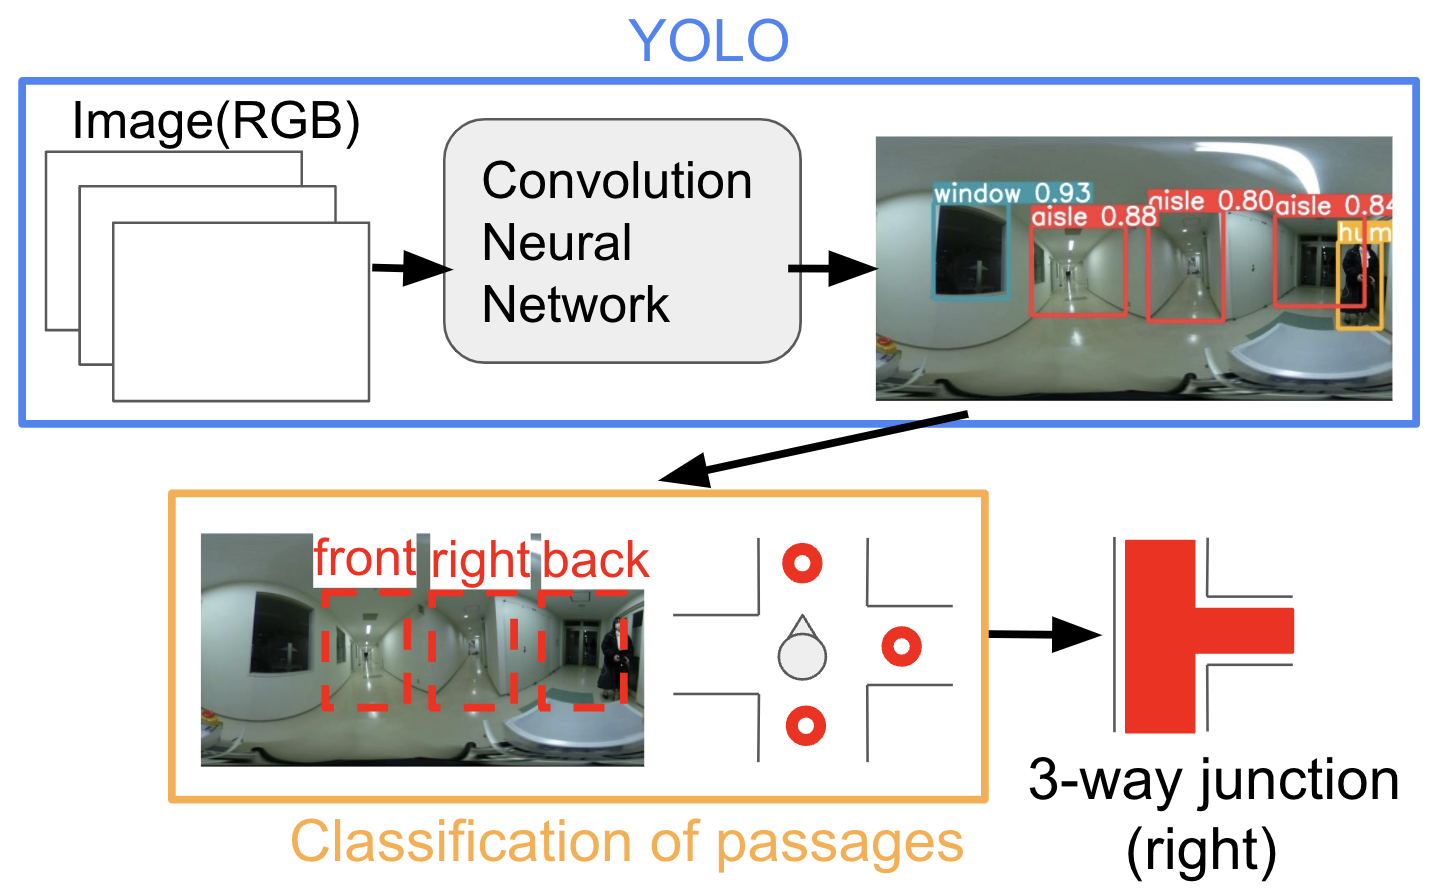
\includegraphics[width=0.45\textwidth]{./fig/fontbig2_proposed_method.png}
        \caption{Conceptual diagram of passage classification method}
        \label{fig:proposed_method}
    \end{figure}
    

    \subsection{データセットの作成}
     学習モデル作成のため,独自に作成したデータセットを用いて学習を行う.
     データセットの画像は津田沼キャンパス2号館3階の廊下で収集した.
     データセットの合計枚数は3554枚で,ラベルは通路,ドア,突き当たりなどの11クラスとした.

     \subsection{学習の結果}
     作成したデータセットを用いてYOLOv5\cite{yolov5}により学習を行う.学習に用いるデータセットは
     トレーニング用3540枚,検証用14枚に割り振る.また,ハイパーパラメータはエポック数300,バッチ数8とした.

    \section{実\hspace{2zw}験}%===========================
     \subsection{実験方法}
     実験環境は\reffig{experiment_point}に示す千葉工業大学津田沼キャンパス2号館3階とした.
     \reffig{experiment_point}の丸い図形で示す箇所にロボットを配置し,各地点により取得した全天球カメラ画像から通路の分類
     ができるかどうか検証する.
     赤と緑の丸の箇所はそれぞれ三叉路と角の通路であり,通路に侵入する際の向きにより
     各通路方向に特徴が変化する.そのため,それらの箇所ではロボットの向きを変え,
     同一箇所でも複数の画像データをキャプチャして検証する.
     本実験では,25箇所・47の画像データで検証を行った.

        \begin{figure}[!b]
            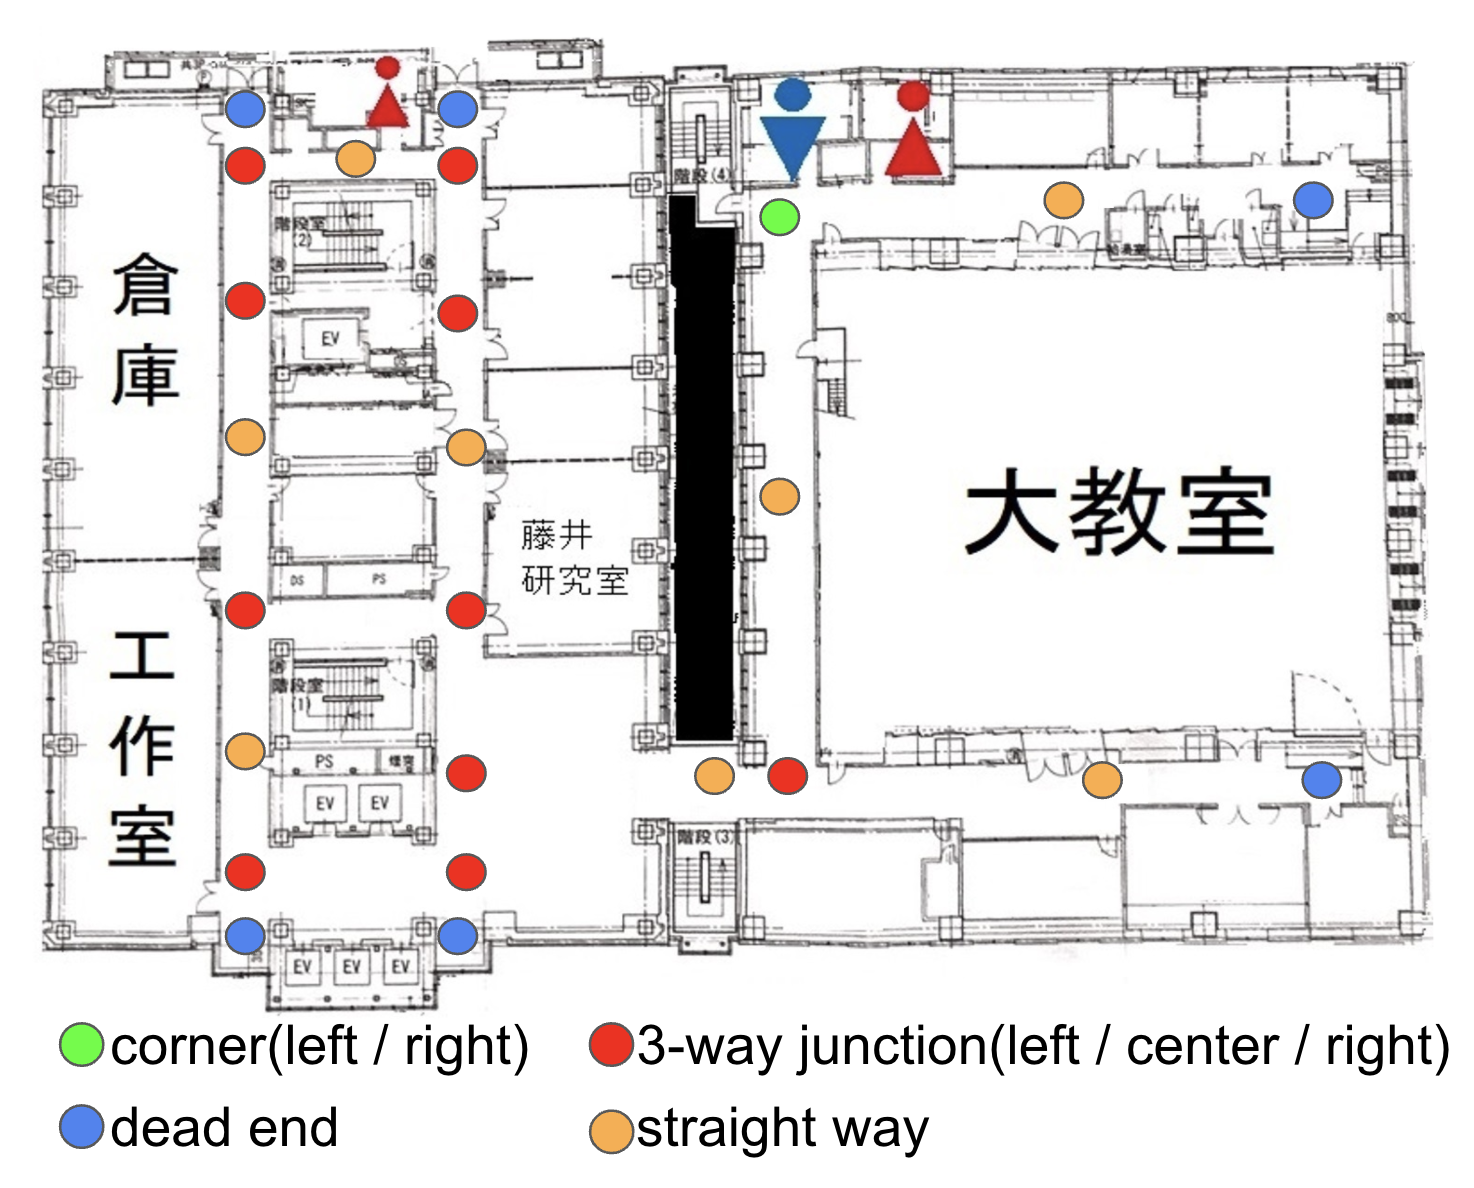
\includegraphics[width=0.46\textwidth]{./fig/new_experimental_point.png}
            \caption{25 point to place robots in aisle classification experiments}
            \label{fig:experiment_point}
        \end{figure}

     \subsection{実験装置}%===========================
     実験装置を\reffig{experiment_machine}に示す.また,図中のカメラを使用する.
    
        \begin{figure}[!b]
            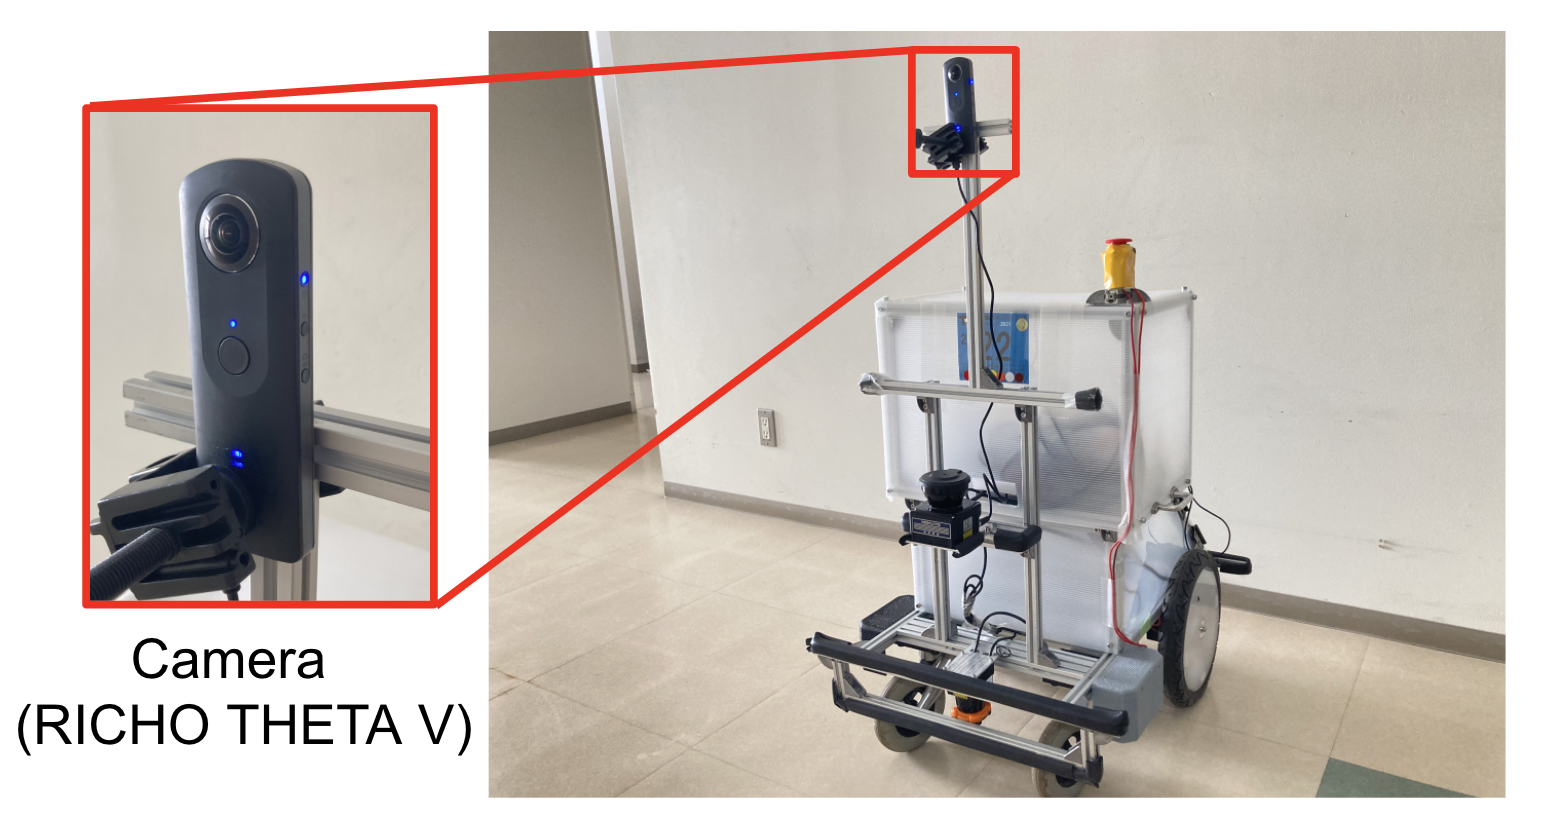
\includegraphics[width=0.46\textwidth]{./fig/experimental_machine_wide.png}
            \caption{The experimental setup machine}
            \label{fig:experiment_machine}
            \end{figure}
    
     \subsection{実験結果}%===========================
     実験の結果,47の画像データの内,42を正しく分類できることが確認できた.
     通路の分類に失敗した箇所は\reffig{miss_classification}に示すように3箇所・5の画像データであり,
     各矢印はロボットの向きを示す.
     失敗の原因は以下の通りで,全て検出器での誤検出が原因であった.\\
     ・1:学習器による後方通路の検出失敗\\
     ・2:学習器により通路を突き当たりと誤検出
     \begin{figure}[!b]
         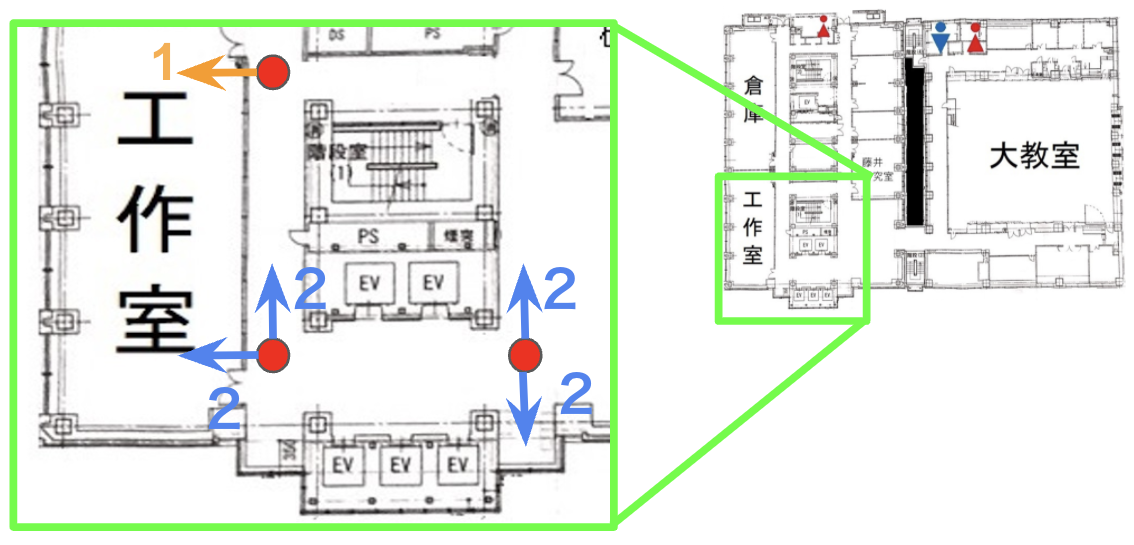
\includegraphics[width=0.46\textwidth]{./fig/experiment_result.png}
         \caption{Points where passage classification failed}
         \label{fig:miss_classification}
     \end{figure}
    
    \section{結\hspace{2zw}言}%===========================
    本研究では,全天球カメラにより取得した水平360度の画像から,YOLOの学習器を用いて通路などの物体検出を行い,
    検出された通路の方向に基づき通路を分類する手法を提案して有効性を検証した.
    結果的に,47例中42例正しく分類できることを確認した.

    
    
    \vspace{5truemm}
    {\footnotesize
        \begin{thebibliography}{5}
            
            \bibitem{shimada_paper1} 島田滉己,上田隆一,林原靖男,”トポロジカルマップを用いたシナリオによるナビゲーションの提案 ー人が道案内に用いる情報の取得と評価ー”,日本機械学会ロボティクス・メカトロニクス講演会'20予稿集,2P1-K02(2020)
            
            \bibitem{shimada_paper2} 島田滉己,上田隆一,林原靖男,”トポロジカルマップを用いたシナリオによるナビゲーションの提案 ーシナリオに基づく実ロボットのナビゲーションー”,1H2-04,SI2020(2020)

            \bibitem{toe_finding_algolithm} Chen,Tongtong,etal.“ Lidar-based long range road intersection detection. ”2011 Sixth International Conferenceon Imageand Graphics.IEEE,(2011)
            \bibitem{yolov5} YOLOv5: https://github.com/ultralytics/yolov5(参照日 \today)
            
        \end{thebibliography}
    }
    \normalsize
    
\end{document}
